\documentclass[aspectratio=169, 12pt]{beamer}
\usepackage{fontspec}
\setmainfont{Arial}

\usetheme{Madrid}
\usecolortheme{default}

\usepackage{graphicx}
\usepackage{amsmath}
\usepackage{listings}
\usepackage{booktabs}
\usepackage{xcolor}
\usepackage{tabularx}
\usepackage{caption}

% Set code listing style
\lstset{
    basicstyle=\ttfamily\scriptsize,
    breaklines=true,
    keywordstyle=\color{blue},
    stringstyle=\color{red},
    commentstyle=\color{green!60!black},
    showstringspaces=false,
    frame=single,
    backgroundcolor=\color{gray!10}
}

\title[ML - Chap 06]{Chương 6: Cây Quyết định (Decision Trees)}
\author[Giảng viên]{Giảng viên}
\institute[Đại học Đông Á]{Đại học Đông Á}
\date{\today}

\begin{document}

% 1
\begin{frame}
    \titlepage
\end{frame}

% 2
\begin{frame}{Mục tiêu của Chương}
    \begin{itemize}
        \item Hiểu rõ thuật toán \textbf{Cây Quyết định (Decision Trees)} và khả năng của nó.
        \item Cách một mô hình cây đưa ra dự đoán (Phân loại và Hồi quy).
        \item Thuật toán \textbf{CART} (Classification and Regression Tree) dùng để huấn luyện.
        \item Tìm hiểu về độ vẩn đục: \textbf{Gini Impurity} và \textbf{Entropy}.
        \item Các kỹ thuật \textbf{Chính quy hóa (Regularization)} bằng siêu tham số.
        \item Điểm yếu của Cây Quyết định: Phương sai cao (High Variance) và nhạy cảm với hướng trục.
    \end{itemize}
\end{frame}

% 3
\begin{frame}{Mục lục}
    \tableofcontents
\end{frame}

%==================================================================
\section{1. Khái quát về Cây Quyết định}
%==================================================================

% 4
\begin{frame}{1.1 Sức mạnh của Decision Trees}
    \begin{itemize}
        \item Cây Quyết định là một trong những thuật toán Học máy đa năng nhất.
        \item Có thể thực hiện cả \textbf{Phân loại (Classification)}, \textbf{Hồi quy (Regression)}, và học nhiều đầu ra (Multioutput).
        \item Khả năng khớp với các tập dữ liệu cực kỳ phức tạp (Non-linear datasets).
        \item Là thành phần cơ bản (Building block) của các thuật toán cực mạnh như \textbf{Random Forest} và \textbf{Gradient Boosting}.
    \end{itemize}
\end{frame}

% 5
\begin{frame}{1.2 Mô hình Hộp Trắng (White Box Model)}
    \begin{itemize}
        \item Điểm sáng giá nhất của Cây Quyết định là tính \textbf{dễ diễn giải (Interpretability)}.
        \item Nó được gọi là mô hình Hộp Trắng (White Box) vì ta có thể theo dõi chính xác cách mô hình đi đến kết luận.
        \item Trái ngược với mô hình Hộp Đen (Black Box) như Mạng nơ-ron hay Random Forest, nơi rất khó giải thích tại sao mô hình lại đưa ra dự đoán đó.
        \item Được sử dụng rộng rãi trong các lĩnh vực Y tế, Tài chính, nơi cần giải trình quyết định.
    \end{itemize}
\end{frame}

%==================================================================
\section{2. Huấn luyện và Trực quan hóa}
%==================================================================

% 6
\begin{frame}[fragile]{2.1 Code: Huấn luyện cây quyết định}
    \begin{itemize}
        \item Sử dụng bộ dữ liệu kinh điển Iris (Hoa diên vĩ).
        \item Ta sẽ chỉ sử dụng 2 đặc trưng: \texttt{petal length} (chiều dài cánh hoa) và \texttt{petal width} (chiều rộng).
    \end{itemize}
\begin{lstlisting}[language=Python]
from sklearn.datasets import load_iris
from sklearn.tree import DecisionTreeClassifier

# Tai tap du lieu Iris
iris = load_iris(as_frame=True)
X_iris = iris.data[["petal length (cm)", "petal width (cm)"]].values
y_iris = iris.target

# Huan luyen mo hinh Cay Quyen dinh
tree_clf = DecisionTreeClassifier(max_depth=2, random_state=42)
tree_clf.fit(X_iris, y_iris)
\end{lstlisting}
\end{frame}

% 7
\begin{frame}[fragile]{2.2 Code: Xuất biểu đồ cây (Graphviz)}
    \begin{itemize}
        \item Scikit-Learn cung cấp phương thức \texttt{export\_graphviz} để vẽ cây thành file \texttt{.dot}.
        \item Sau đó dùng Graphviz để chuyển \texttt{.dot} thành ảnh PNG hoặc PDF.
    \end{itemize}
\begin{lstlisting}[language=Python]
from sklearn.tree import export_graphviz

export_graphviz(
    tree_clf,
    out_file="iris_tree.dot",
    feature_names=["petal length (cm)", "petal width (cm)"],
    class_names=iris.target_names,
    rounded=True,
    filled=True
)
# Lenh terminal bien dich dot sang png:
# dot -Tpng iris_tree.dot -o iris_tree.png
\end{lstlisting}
\end{frame}

% 8
\begin{frame}{2.3 Trực quan hóa Cây Iris}
    \begin{columns}
        \begin{column}{0.4\textwidth}
            \begin{itemize}
                \item Nút trên cùng gọi là \textbf{Nút gốc (Root Node)}.
                \item Nút không có con gọi là \textbf{Nút lá (Leaf Node)}.
                \item Mỗi nút hiển thị: Điều kiện chia, số \texttt{samples} (mẫu), \texttt{value} (phân bố), và \texttt{class} (nhãn dự đoán).
            \end{itemize}
        \end{column}
        \begin{column}{0.6\textwidth}
            \centering
            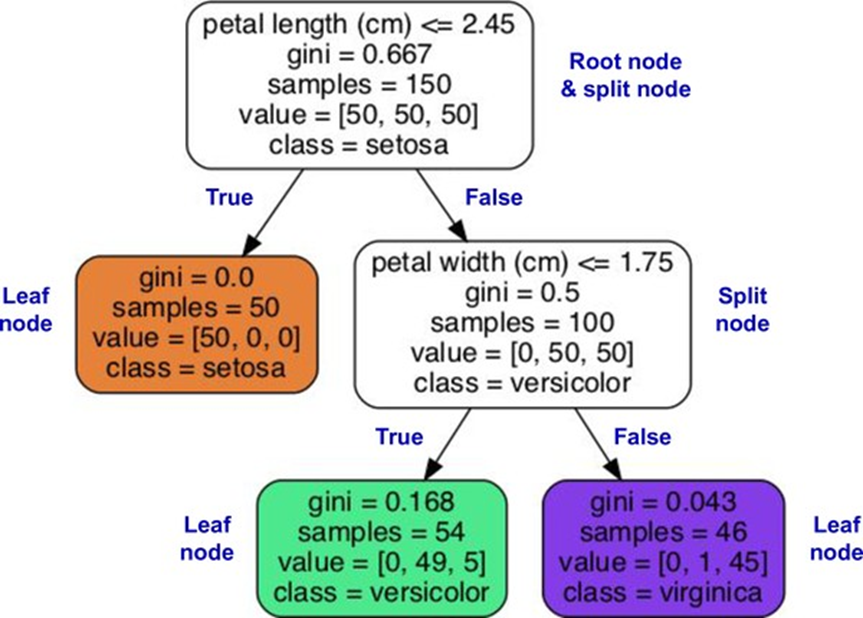
\includegraphics[width=\textwidth,height=0.7\textheight,keepaspectratio]{../machineLearningWeb/Figures/CH06/Hinh_6-1.png}
            \vspace{0.1cm}
            \captionof{figure}{Hình 6-1: Cây Quyết định bộ dữ liệu Iris}
        \end{column}
    \end{columns}
\end{frame}

%==================================================================
\section{3. Đưa ra dự đoán (Making Predictions)}
%==================================================================

% 9
\begin{frame}{3.1 Quá trình đưa ra dự đoán}
    \begin{itemize}
        \item Cây sẽ duyệt từ \textbf{Nút gốc} đi xuống.
        \item Ở mỗi nút, nó kiểm tra một điều kiện (VD: petal\_length $\le$ 2.45 cm).
        \item Nếu \textbf{Đúng (True)}, đi sang nhánh bên Trái.
        \item Nếu \textbf{Sai (False)}, đi sang nhánh bên Phải.
        \item Lặp lại đến khi gặp Nút lá. Lớp có số lượng mẫu đông nhất trong nút lá đó sẽ là dự đoán cuối cùng.
    \end{itemize}
\end{frame}

% 10
\begin{frame}{3.2 Hiểu về Gini Impurity (Độ vẩn đục Gini)}
    \begin{itemize}
        \item Tham số \texttt{gini} ở mỗi nút đo lường \textbf{độ vẩn đục} (impurity) của nó.
        \item Một nút được gọi là "thuần khiết" (pure) nếu $gini = 0$, nghĩa là mọi mẫu trong nút đó đều thuộc về \textbf{cùng một lớp}.
        \item Công thức Gini Impurity cho nút $i$:
        $$ G_i = 1 - \sum_{k=1}^{n} p_{i,k}^2 $$
        \item Trong đó: $p_{i,k}$ là tỷ lệ phần trăm mẫu thuộc lớp $k$ nằm trong nút $i$.
    \end{itemize}
\end{frame}

% 11
\begin{frame}{3.3 Ví dụ tính toán Gini Impurity}
    \begin{itemize}
        \item Xem lại Hình 6-1, Nút màu xanh lục (phía dưới bên trái):
        \item Có tổng cộng 54 mẫu. Lớp Setosa (0), Lớp Versicolor (49), Lớp Virginica (5).
        \item Tỷ lệ $p$: $p_{versicolor} = 49/54$, $p_{virginica} = 5/54$.
        \item Áp dụng công thức:
        $$ G_i = 1 - \left(\left(\frac{0}{54}\right)^2 + \left(\frac{49}{54}\right)^2 + \left(\frac{5}{54}\right)^2\right) $$
        $$ G_i \approx 1 - (0 + 0.823 + 0.008) \approx 0.168 $$
    \end{itemize}
\end{frame}

% 12
\begin{frame}{3.4 Ranh giới Quyết định (Decision Boundaries)}
    \begin{columns}
        \begin{column}{0.4\textwidth}
            \begin{itemize}
                \item Hình ảnh minh họa không gian đặc trưng.
                \item Đường nét đậm ở 2.45 cm (Trục tung) là ranh giới từ nút gốc.
                \item Đường đứt nét ở 1.75 cm (Trục hoành) là ranh giới chia nhánh thứ hai.
                \item Cây luôn tạo ra các đường ranh giới \textbf{vuông góc với trục tọa độ}.
            \end{itemize}
        \end{column}
        \begin{column}{0.6\textwidth}
            \centering
            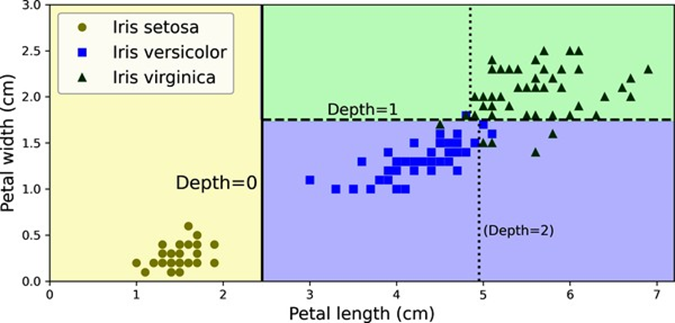
\includegraphics[width=\textwidth,height=0.7\textheight,keepaspectratio]{../machineLearningWeb/Figures/CH06/Hinh_6-2.png}
            \vspace{0.1cm}
            \captionof{figure}{Hình 6-2: Ranh giới quyết định của Cây}
        \end{column}
    \end{columns}
\end{frame}

% 13
\begin{frame}{3.5 Không cần Chuẩn hóa (Scaling) dữ liệu!}
    \begin{itemize}
        \item Một ưu điểm tuyệt vời khác của Cây Quyết định: \textbf{Nó gần như không yêu cầu tiền xử lý dữ liệu!}
        \item Không cần \texttt{StandardScaler} hay \texttt{MinMaxScaler}.
        \item Việc một đặc trưng chạy từ 0-1 còn đặc trưng khác chạy từ 0-1000 không hề ảnh hưởng đến việc phân chia nhánh. Thuật toán chỉ tìm điểm ngưỡng cắt $t_k$.
    \end{itemize}
\end{frame}

% 14
\begin{frame}{3.6 Ước tính Xác suất Lớp (Class Probabilities)}
    \begin{itemize}
        \item Cây quyết định cũng có thể trả về \textbf{xác suất} mà một mẫu thuộc về một lớp cụ thể.
        \item Bằng cách duyệt từ gốc xuống một nút lá.
        \item Xác suất của lớp $k$ chính là tỉ lệ mẫu của lớp $k$ trên tổng số mẫu tại nút lá đó.
        \item VD: Bông hoa dài 5cm, rộng 1.5cm sẽ đi vào nút lá màu xanh lục (49 Versicolor, 5 Virginica). Xác suất là $49/54 \approx 90.7\%$ cho Versicolor.
    \end{itemize}
\end{frame}

% 15
\begin{frame}[fragile]{3.7 Code: Dự đoán Xác suất}
\begin{lstlisting}[language=Python]
# Du doan xac suat cho 1 bong hoa:
# petal_length = 5.0, petal_width = 1.5
probabilities = tree_clf.predict_proba([[5, 1.5]])
print("Xac suat (Setosa, Versi, Virgi):", probabilities)
# Output: [[0.         0.90740741 0.09259259]]

# Du doan lop (argmax cua xac suat)
pred_class = tree_clf.predict([[5, 1.5]])
print("Lop du doan:", pred_class)
# Output: [1] (tuc la Versicolor)
\end{lstlisting}
\end{frame}


%==================================================================
\section{4. Thuật toán Huấn luyện CART}
%==================================================================

% 16
\begin{frame}{4.1 Thuật toán CART là gì?}
    \begin{itemize}
        \item Scikit-Learn sử dụng thuật toán \textbf{CART} (Classification and Regression Tree) để huấn luyện cây.
        \item Thuật toán này khá đơn giản:
        \begin{enumerate}
            \item Phân chia tập huấn luyện thành 2 tập con sử dụng 1 đặc trưng $k$ và ngưỡng $t_k$.
            \item Chọn $k$ và $t_k$ sao cho tạo ra 2 tập con thuần khiết nhất (tức là Gini Impurity nhỏ nhất có thể).
            \item Lặp lại đệ quy với từng tập con.
            \item Dừng lại khi đạt đến \texttt{max\_depth} hoặc không thể giảm thêm độ vẩn đục.
        \end{enumerate}
    \end{itemize}
\end{frame}

% 17
\begin{frame}{4.2 Hàm Chi phí của CART (Phân loại)}
    \begin{itemize}
        \item Thuật toán CART sẽ tối thiểu hóa hàm chi phí (Cost Function) tại mỗi bước chia:
        $$ J(k, t_k) = \frac{m_{left}}{m} G_{left} + \frac{m_{right}}{m} G_{right} $$
        \item Trong đó:
        \begin{itemize}
            \item $G_{left}, G_{right}$ là độ vẩn đục Gini của tập con bên trái/phải.
            \item $m_{left}, m_{right}$ là số lượng mẫu của tập con.
            \item $m$ là tổng số lượng mẫu tại nút đang xét.
        \end{itemize}
        \item CART là thuật toán \textbf{Tham lam (Greedy Algorithm)}. Nó chỉ tìm kiếm mức phân tách tốt nhất tại \textit{hiện tại}, không nhìn về tương lai. Do đó không bảo đảm tối ưu cục bộ.
    \end{itemize}
\end{frame}

% 18
\begin{frame}{4.3 Gini Impurity hay Information Entropy?}
    \begin{itemize}
        \item Mặc định, CART dùng \textbf{Gini Impurity} (\texttt{criterion="gini"}).
        \item Tuy nhiên, ta có thể đổi sang dùng \textbf{Entropy} (\texttt{criterion="entropy"}).
        \item Entropy bằng $0$ khi tập hợp hoàn toàn thuần khiết (chỉ chứa 1 lớp).
        \item Công thức Shannon's Entropy:
        $$ H_i = -\sum_{k=1, p_{i,k} \neq 0}^{n} p_{i,k} \log_2(p_{i,k}) $$
    \end{itemize}
\end{frame}

% 19
\begin{frame}{4.4 So sánh Gini và Entropy}
    \begin{itemize}
        \item Vậy nên sử dụng cái nào?
        \item Hầu hết mọi trường hợp, \textbf{Gini và Entropy tạo ra những cây rất giống nhau}.
        \item Gini tính toán \textbf{nhanh hơn một chút} (vì không chứa phép Logarit), là lựa chọn mặc định tốt.
        \item Entropy đôi khi có xu hướng tạo ra các cây cân bằng hơn (balanced trees) trong khi Gini thường cắt ra nhánh lớn nhất.
    \end{itemize}
\end{frame}

% 20
\begin{frame}{4.5 Độ phức tạp Thời gian (Time Complexity)}
    \begin{itemize}
        \item \textbf{Quá trình Suy luận (Dự đoán):}
        \begin{itemize}
            \item Phải duyệt từ gốc đến lá. Độ sâu là $O(\log_2(m))$.
            \item Phức tạp dự đoán cực nhanh: $O(\log_2(m))$ độc lập với số lượng đặc trưng!
        \end{itemize}
        \item \textbf{Quá trình Huấn luyện:}
        \begin{itemize}
            \item Thuật toán so sánh mọi đặc trưng (hoặc \texttt{max\_features} nếu được cài) trên mọi ngưỡng.
            \item Phức tạp thời gian là $O(n \times m \log_2(m))$.
            \item Rất chậm đối với các tập dữ liệu có $m$ lớn (Hàng triệu dòng).
        \end{itemize}
    \end{itemize}
\end{frame}


%==================================================================
\section{5. Chính quy hóa Cây (Regularization)}
%==================================================================

% 21
\begin{frame}{5.1 Tại sao phải Chính quy hóa?}
    \begin{itemize}
        \item Cây quyết định là mô hình \textbf{Non-parametric} (Phi tham số).
        \item Nghĩa là số lượng tham số không được ấn định trước, dẫn đến việc mô hình có thể phát triển tự do theo dữ liệu.
        \item Nếu không có giới hạn, cây sẽ cố phân nhánh đến khi mỗi chiếc lá chỉ có 1 điểm duy nhất (Tương đương việc ghi nhớ học vẹt bộ dữ liệu).
        \item Điều này gây ra hiện tượng \textbf{Overfitting} cực kỳ nghiêm trọng.
    \end{itemize}
\end{frame}

% 22
\begin{frame}{5.2 Các Siêu tham số Chính quy hóa}
    \begin{itemize}
        \item \texttt{max\_depth}: Độ sâu tối đa của cây (Default: None). Giảm nó để hạn chế Overfitting.
        \item \texttt{min\_samples\_split}: Số lượng mẫu tối thiểu một nút phải có trước khi được phân chia.
        \item \texttt{min\_samples\_leaf}: Số mẫu tối thiểu một nút lá phải có.
        \item \texttt{max\_leaf\_nodes}: Số lượng nút lá tối đa.
        \item \texttt{max\_features}: Số lượng đặc trưng tối đa được xem xét tại mỗi lần chia.
    \end{itemize}
\end{frame}

% 23
\begin{frame}{5.3 Hiệu ứng của Chính quy hóa}
    \begin{columns}
        \begin{column}{0.4\textwidth}
            \begin{itemize}
                \item Hình bên trái: Cây không giới hạn (\texttt{min\_samples\_leaf=1}). Ranh giới ngoằn ngoèo, Overfitting.
                \item Hình bên phải: Cây bị ràng buộc (\texttt{min\_samples\_leaf=4}). Ranh giới mượt mà hơn, khả năng tổng quát hóa (Generalization) tốt hơn trên dữ liệu mới.
            \end{itemize}
        \end{column}
        \begin{column}{0.6\textwidth}
            \centering
            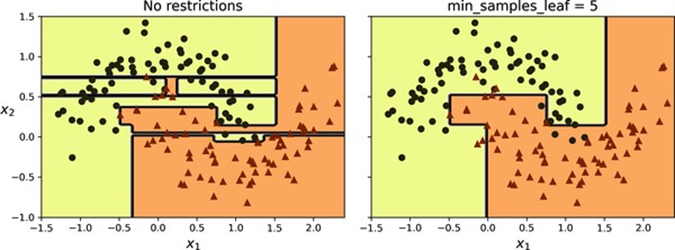
\includegraphics[width=\textwidth,height=0.7\textheight,keepaspectratio]{../machineLearningWeb/Figures/CH06/Hinh_6-3.png}
            \vspace{0.1cm}
            \captionof{figure}{Hình 6-3: Cây không chính quy (trái) vs Chính quy hóa (phải)}
        \end{column}
    \end{columns}
\end{frame}


%==================================================================
\section{6. Hồi quy bằng Cây quyết định}
%==================================================================

% 24
\begin{frame}{6.1 Lớp DecisionTreeRegressor}
    \begin{itemize}
        \item Cây quyết định cũng giải quyết xuất sắc các bài toán Hồi quy.
        \item Lúc này, thay vì dự đoán một "nhãn lớp", nút lá sẽ dự đoán một "giá trị liên tục" (Trung bình cộng của tất cả các mẫu nằm trong lá đó).
        \item Sử dụng hàm mục tiêu là MSE (Mean Squared Error) để tối ưu.
    \end{itemize}
\end{frame}

% 25
\begin{frame}[fragile]{6.2 Code: Hồi quy dữ liệu Quadratic}
\begin{lstlisting}[language=Python]
import numpy as np
from sklearn.tree import DecisionTreeRegressor

# Tao du lieu mo phong y = x^2 + nhieu
np.random.seed(42)
X_quad = np.random.rand(200, 1) - 0.5
y_quad = X_quad ** 2 + 0.025 * np.random.randn(200, 1)

# Huan luyen cay hoi quy (Gioi han max_depth)
tree_reg = DecisionTreeRegressor(max_depth=2, random_state=42)
tree_reg.fit(X_quad, y_quad)
\end{lstlisting}
\end{frame}

% 26
\begin{frame}{6.3 Trực quan hóa Cây Hồi quy}
    \begin{columns}
        \begin{column}{0.4\textwidth}
            \begin{itemize}
                \item Hình bên minh họa cây Hồi quy độ sâu 2.
                \item Ở mỗi nút lá, giá trị \texttt{value} chính là $y$ trung bình của các mẫu, và \texttt{mse} (Mean Squared Error) là sai số tại nút đó.
                \item Dự đoán sẽ mang dạng các \textbf{bậc thang (step-wise)} vì trong cùng 1 khoảng chia, mọi giá trị x đều trả ra cùng 1 mức y.
            \end{itemize}
        \end{column}
        \begin{column}{0.6\textwidth}
            \centering
            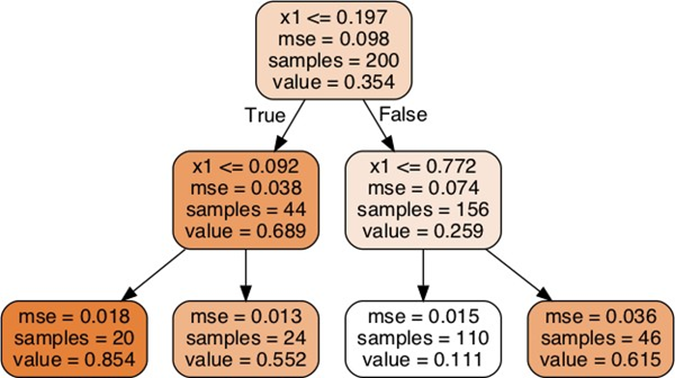
\includegraphics[width=\textwidth,height=0.7\textheight,keepaspectratio]{../machineLearningWeb/Figures/CH06/Hinh_6-4.png}
            \vspace{0.1cm}
            \captionof{figure}{Hình 6-4: Sơ đồ Decision Tree Regression}
        \end{column}
    \end{columns}
\end{frame}

% 27
\begin{frame}{6.4 Các Ranh giới Hồi quy (Bậc thang)}
    \begin{columns}
        \begin{column}{0.4\textwidth}
            \begin{itemize}
                \item Trái: \texttt{max\_depth = 2} (Có 4 bậc thang).
                \item Phải: \texttt{max\_depth = 3} (Có 8 bậc thang).
                \item Cây phân chia không gian thành các mảng và dự đoán $y$ là đường thẳng hằng số trên từng mảng.
            \end{itemize}
        \end{column}
        \begin{column}{0.6\textwidth}
            \centering
            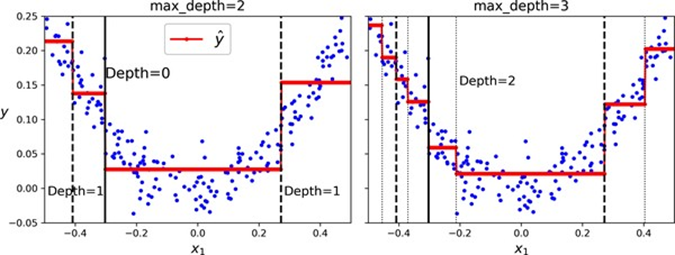
\includegraphics[width=\textwidth,height=0.7\textheight,keepaspectratio]{../machineLearningWeb/Figures/CH06/Hinh_6-5.png}
            \vspace{0.1cm}
            \captionof{figure}{Hình 6-5: Hàm dự đoán của Cây Hồi quy}
        \end{column}
    \end{columns}
\end{frame}

% 28
\begin{frame}{6.5 Overfitting trong Hồi quy}
    \begin{itemize}
        \item Tương tự như phân loại, Cây Hồi quy rất dễ bị Overfitting nếu không ràng buộc.
        \item Cây sẽ uốn éo đứt đoạn để đi qua toàn bộ các nhiễu dữ liệu.
        \item Khắc phục: Dùng \texttt{min\_samples\_leaf=10} để ép mô hình mượt mà hơn.
    \end{itemize}
\end{frame}

% 29
\begin{frame}{6.6 Hàm Chi phí CART cho Hồi quy}
    \begin{itemize}
        \item Thuật toán CART sẽ tối thiểu hóa sai số MSE thay vì Gini Impurity:
        $$ J(k, t_k) = \frac{m_{left}}{m} \text{MSE}_{left} + \frac{m_{right}}{m} \text{MSE}_{right} $$
        \item Trong đó:
        $$ \text{MSE}_{node} = \frac{1}{m_{node}} \sum_{i \in node} (\hat{y}_{node} - y^{(i)})^2 $$
        \item Và $\hat{y}_{node}$ luôn là Trung bình cộng của các mẫu trong lá.
    \end{itemize}
\end{frame}


%==================================================================
\section{7. Các Điểm yếu của Cây Quyết Định}
%==================================================================

% 30
\begin{frame}{7.1 Trục chia vuông góc (Orthogonal splits)}
    \begin{itemize}
        \item Cây quyết định yêu thích sự đơn giản. Nó luôn phân chia tập dữ liệu bằng các đường \textbf{song song hoặc vuông góc} với trục tọa độ.
        \item Nó không thể vẽ đường chéo hay đường cong!
        \item Điều này dẫn đến sự nhạy cảm cực độ đối với \textbf{Hướng Xoay của Dữ liệu (Axis Orientation)}.
    \end{itemize}
\end{frame}

% 31
\begin{frame}{7.2 Nhạy cảm với Xoay trục tọa độ}
    \begin{columns}
        \begin{column}{0.45\textwidth}
            \begin{itemize}
                \item Hình Trái: Dữ liệu phân tách tuyệt đẹp bằng 1 đường thẳng ngang. (Cây sâu 1 tầng).
                \item Hình Phải: Cùng bộ dữ liệu nhưng xoay 45 độ. Cây buộc phải chia cắt thành vô vàn đường cầu thang ziczac dốc để xấp xỉ một đường chéo.
                \item Cây rườm rà, tổng quát hóa kém.
            \end{itemize}
        \end{column}
        \begin{column}{0.55\textwidth}
            \centering
            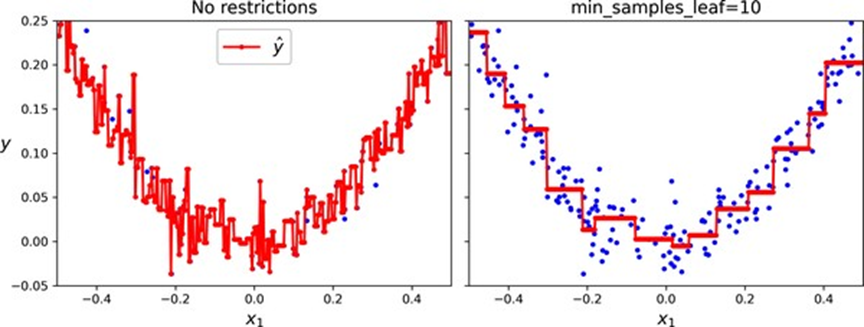
\includegraphics[width=\textwidth,height=0.65\textheight,keepaspectratio]{../machineLearningWeb/Figures/CH06/Hinh_6-6.png}
            \vspace{0.1cm}
            \captionof{figure}{Hình 6-6: Độ nhạy cảm với trục xoay dữ liệu}
        \end{column}
    \end{columns}
\end{frame}

% 32
\begin{frame}{7.3 Khắc phục Bằng PCA (Phân tích Thành phần Chính)}
    \begin{columns}
        \begin{column}{0.45\textwidth}
            \begin{itemize}
                \item Để giảm bớt sự nhạy cảm, ta có thể kết hợp Tiền xử lý bằng PCA (Principal Component Analysis).
                \item PCA sẽ xoay tập dữ liệu về trạng thái mà phương sai là lớn nhất trên các trục tọa độ.
                \item Nhờ đó, giới hạn khả năng cây bị bóp méo đường cầu thang.
            \end{itemize}
        \end{column}
        \begin{column}{0.55\textwidth}
            \centering
            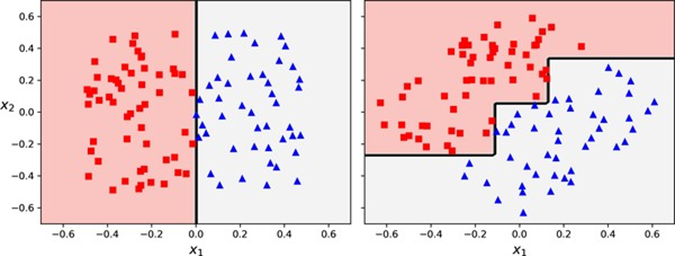
\includegraphics[width=\textwidth,height=0.65\textheight,keepaspectratio]{../machineLearningWeb/Figures/CH06/Hinh_6-7.png}
            \vspace{0.1cm}
            \captionof{figure}{Hình 6-7: Cây phân loại sau khi xoay bằng PCA}
        \end{column}
    \end{columns}
\end{frame}

% 33
\begin{frame}{7.4 Phương sai cao (High Variance)}
    \begin{itemize}
        \item Vấn đề lớn nhất của Cây Quyết định: \textbf{Tính không ổn định cực cao (High Variance)}.
        \item Vì là một thuật toán tham lam (không kiểm tra lại toàn bộ tương lai), một \textbf{thay đổi vô cùng nhỏ} trong tập huấn luyện có thể tạo ra một cây \textbf{hoàn toàn khác biệt}.
        \item Một nhiễu loạn ngẫu nhiên nhỏ xíu ở nút gốc sẽ làm toàn bộ các nút con thay đổi.
    \end{itemize}
\end{frame}

% 34
\begin{frame}{7.5 Ví dụ về High Variance}
    \begin{columns}
        \begin{column}{0.45\textwidth}
            \begin{itemize}
                \item Trong bộ dữ liệu Iris, giả sử ta xóa \textbf{đúng 1 bông hoa} Versicolor to nhất (Dài 4.8cm, rộng 1.8cm).
                \item Cây mới học được (Bên phải) đã chia cắt dữ liệu theo ranh giới khác hoàn toàn so với cây ban đầu (Hình 6-2).
            \end{itemize}
        \end{column}
        \begin{column}{0.55\textwidth}
            \centering
            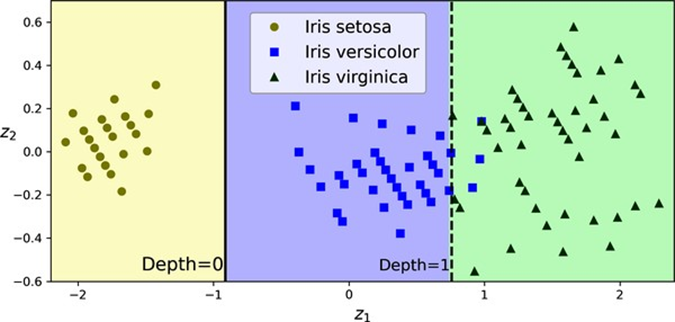
\includegraphics[width=\textwidth,height=0.7\textheight,keepaspectratio]{../machineLearningWeb/Figures/CH06/Hinh_6-8.png}
            \vspace{0.1cm}
            \captionof{figure}{Hình 6-8: Cây bị méo mó chỉ sau khi xóa 1 điểm}
        \end{column}
    \end{columns}
\end{frame}

% 35
\begin{frame}{7.6 Ngẫu nhiên tính trong Huấn luyện}
    \begin{itemize}
        \item Ngay cả khi bạn \textbf{không xóa} bất kỳ dữ liệu nào, bản thân Scikit-Learn cũng chọn đặc trưng theo cách \textbf{ngẫu nhiên} để tăng tốc độ phân chia.
        \item Nghĩa là, huấn luyện cùng 1 tập dữ liệu 2 lần có thể ra 2 kết quả khác nhau (Nếu không set \texttt{random\_state=42}).
        \item Sự ngẫu nhiên và Phương sai cao này thoạt nghe có vẻ là điểm yếu chí mạng...
    \end{itemize}
\end{frame}

% 36
\begin{frame}{7.7 Từ Điểm yếu trở thành Siêu Vị Thần (Random Forest)}
    \begin{columns}
        \begin{column}{0.45\textwidth}
            \begin{itemize}
                \item Thay vì dùng 1 cái cây không ổn định, ta sẽ trồng hàng nghìn cái cây như thế!
                \item Bằng cách trung bình hóa dự đoán của một \textbf{Khu Rừng (Forest)} các cây có phương sai cao và độc lập nhau.
                \item Kết quả là thuật toán \textbf{Random Forest} - một trong những thuật toán ML vĩ đại nhất lịch sử ra đời!
            \end{itemize}
        \end{column}
        \begin{column}{0.55\textwidth}
            \centering
            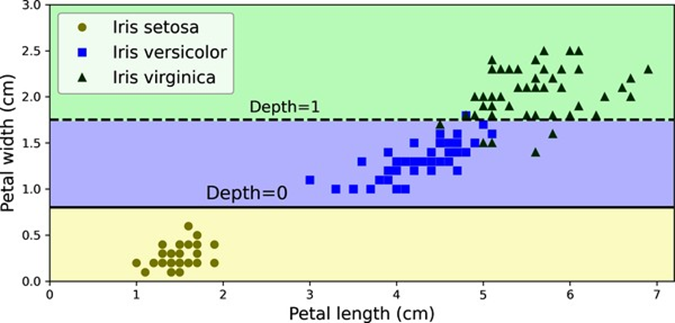
\includegraphics[width=\textwidth,height=0.65\textheight,keepaspectratio]{../machineLearningWeb/Figures/CH06/Hinh_6-9.png}
            \vspace{0.1cm}
            \captionof{figure}{Hình 6-9: Khu rừng Random Forest (Chương 7)}
        \end{column}
    \end{columns}
\end{frame}


%==================================================================
\section{8. Tổng kết}
%==================================================================

% 37
\begin{frame}{8.1 Ưu điểm tóm tắt}
    \begin{itemize}
        \item \textbf{Dễ hiểu, Dễ giải thích:} Có thể xuất ra dạng quy tắc (If-Else) hoặc sơ đồ luồng.
        \item \textbf{Không yêu cầu Chuẩn hóa:} Hoạt động tốt ngay cả khi các biến khác đơn vị, hoặc lẫn lộn chữ và số.
        \item \textbf{Xử lý Phi tuyến tính:} Cắt xẻ không gian tọa độ cực tốt, khớp với ranh giới phức tạp.
        \item \textbf{Nhanh ở khâu Dự đoán:} Suy luận với tốc độ Logarit $O(\log_2 m)$.
    \end{itemize}
\end{frame}

% 38
\begin{frame}{8.2 Nhược điểm tóm tắt}
    \begin{itemize}
        \item \textbf{Overfitting nặng nề:} Thích ôm chặt lấy dữ liệu huấn luyện nếu không bị kìm hãm bằng Regularization.
        \item \textbf{Nhạy cảm với Xoay trục:} Bị trói buộc vào các ranh giới song song trục tọa độ (Khắc phục bằng PCA).
        \item \textbf{Instability (Bất ổn / Variance Cao):} Rung lắc mạnh khi dữ liệu chỉ đổi một tẹo. (Khắc phục bằng Ensemble Learning).
    \end{itemize}
\end{frame}

% 39
\begin{frame}{8.3 Bài tập 1: Phân loại Moons}
    \begin{itemize}
        \item Khởi tạo bộ dữ liệu 10.000 điểm bằng \texttt{make\_moons(n\_samples=10000, noise=0.4)}.
        \item Phân chia thành Train/Test bằng \texttt{train\_test\_split}.
        \item Dùng \texttt{GridSearchCV} với \texttt{DecisionTreeClassifier} để dò tìm siêu tham số \texttt{max\_leaf\_nodes} tốt nhất.
        \item Huấn luyện và tính Accuracy Score.
    \end{itemize}
\end{frame}

% 40
\begin{frame}{8.4 Bài tập 2: Tự xây dựng Khu rừng (Forest)}
    \begin{itemize}
        \item Bổ sung từ Bài tập 1. Thay vì 1 cây, hãy tạo 1000 tập con dữ liệu từ Train set.
        \item Dùng vòng lặp huấn luyện 1000 Cây Quyết Định (với cấu hình tốt nhất từ Bài 1) trên mỗi tập con.
        \item Dự đoán trên Test set: Bằng cách áp dụng \textbf{Mode} (Lấy dự đoán được số đông vote nhiều nhất) từ 1000 cây cho mỗi mẫu.
        \item Độ chính xác của bạn sẽ tăng hơn ít nhất $0.5 - 1.5\%$ so với 1 cây.
    \end{itemize}
\end{frame}

% 41
\begin{frame}
    \centering
    \Huge \textbf{HỎI \& ĐÁP}
\end{frame}

\end{document}
